\documentclass[12pt]{article}
\setlength{\oddsidemargin}{0in}
\setlength{\evensidemargin}{0in}
\setlength{\textwidth}{6.5in}
\setlength{\parindent}{0in}
\setlength{\parskip}{\baselineskip}
\usepackage{amsmath,amsfonts,amssymb}
\usepackage{graphicx}
\usepackage{enumitem}
\usepackage[]{algorithmicx}
\usepackage{amsthm}
\usepackage{fancyhdr}
\pagestyle{fancy}
\setlength{\headsep}{36pt}
\usepackage{tkz-berge}
\usetikzlibrary{positioning, automata}

\usepackage{hyperref}

\theoremstyle{remark}
\newtheorem*{solution}{Solution}

\newcommand{\makenonemptybox}[2]{%
%\par\nobreak\vspace{\ht\strutbox}\noindent
\item[]
\fbox{% added -2\fboxrule to specified width to avoid overfull hboxes
% and removed the -2\fboxsep from height specification (image not updated)
% because in MWE 2cm is should be height of contents excluding sep and frame
\parbox[c][#1][t]{\dimexpr\linewidth-2\fboxsep-2\fboxrule}{
  \hrule width \hsize height 0pt
  #2
 }%
}%
\par\vspace{\ht\strutbox}
}
\makeatother

\begin{document}
\definecolor {processblue}{cmyk}{0.96,0,0,0}

\lhead{{\bf CSCI 3104, Algorithms \\ Problem Set 5a (11 points)} }
\rhead{Name: Luna McBride \\ ID: 107607144 \\ {\bf Profs.\ Hoenigman \& Agrawal\\ Fall 2019, CU-Boulder}}
\renewcommand{\headrulewidth}{0.5pt}

\phantom{Test}

\begin{small}
\textbf{Instructions for submitting your solution}:
\vspace{-5mm} 

\begin{itemize}
	\item The solutions \textbf{should be typed} and we cannot accept hand-written solutions. \href{http://ece.uprm.edu/~caceros/latex/introduction.pdf}{Here's a short intro to Latex.}
	\item You should submit your work through \href{https://www.gradescope.com/courses/59294}{\textbf{Gradescope}} only.
	\item If you don't have an account on it, sign up for one using your CU email. You should have gotten an email to sign up. If your name based CU email doesn't work, try the identikey@colorado.edu version. 
	\item Gradescope will only accept \textbf{.pdf} files (except for code files that should be submitted separately on Gradescope if a problem set has them) and \textbf{try to fit your work in the box provided}. 
	\item You cannot submit a pdf which has less pages than what we provided you as Gradescope won't allow it. 
	\item Verbal reasoning is typically insufficient for full credit. Instead, write a logical argument, in the style of a mathematical proof.
	\item For every problem in this class, you must justify your answer:\ show how you arrived at it and why it is correct. If there are assumptions you need to make along the way, state those clearly.
	
	\item You may work with other students. However, \textbf{all solutions must be written independently and in your own words.} Referencing solutions of any sort is strictly prohibited. You must explicitly cite any sources, as well as any collaborators. 
\end{itemize}



\vspace{-4mm} 
\end{small}

\hrulefill

\newpage
\begin{enumerate}
%\item (2 pt) Use the following graph $G$ to describe the difference between an MST and the single-source shortest path in a graph. Your answer should clearly describe the different trees that Kruskals and Dijkstras algorithms produce on $G$. 
\item (7 pts) Consider the following weighted graph. 
\begin{figure}[h!]
\begin{center}
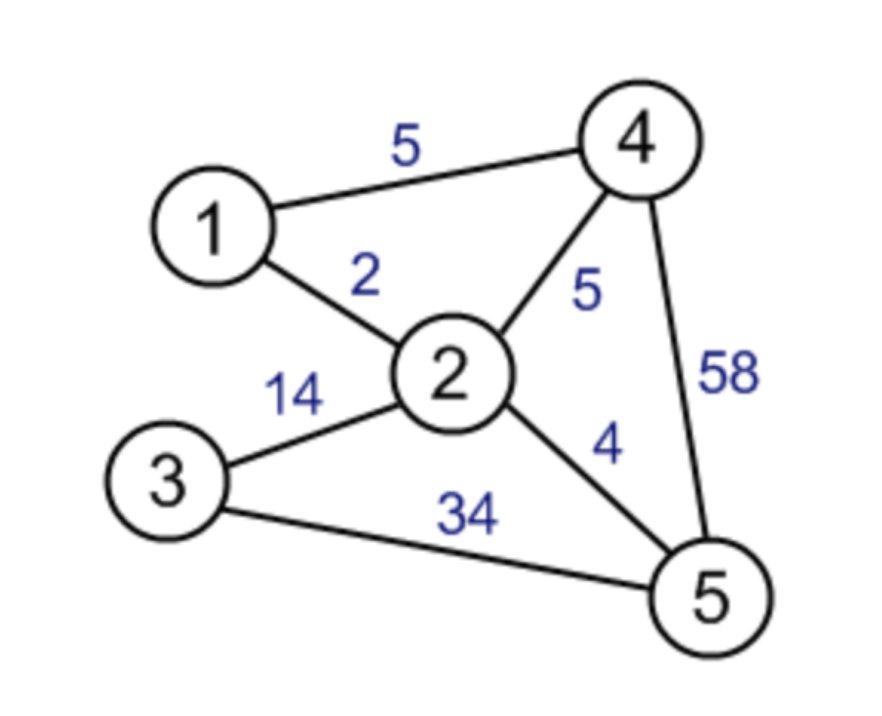
\includegraphics[scale=0.3]{PS5aQ1.png} 
\end{center}
\end{figure}

\begin{enumerate}[label=(\alph*)]
\item (2 pts) Run Dijkstra's algorithm on this graph to obtain a tree of shortest paths. Use vertex $1$ as the source vertex.
\begin{solution}
$\newline$$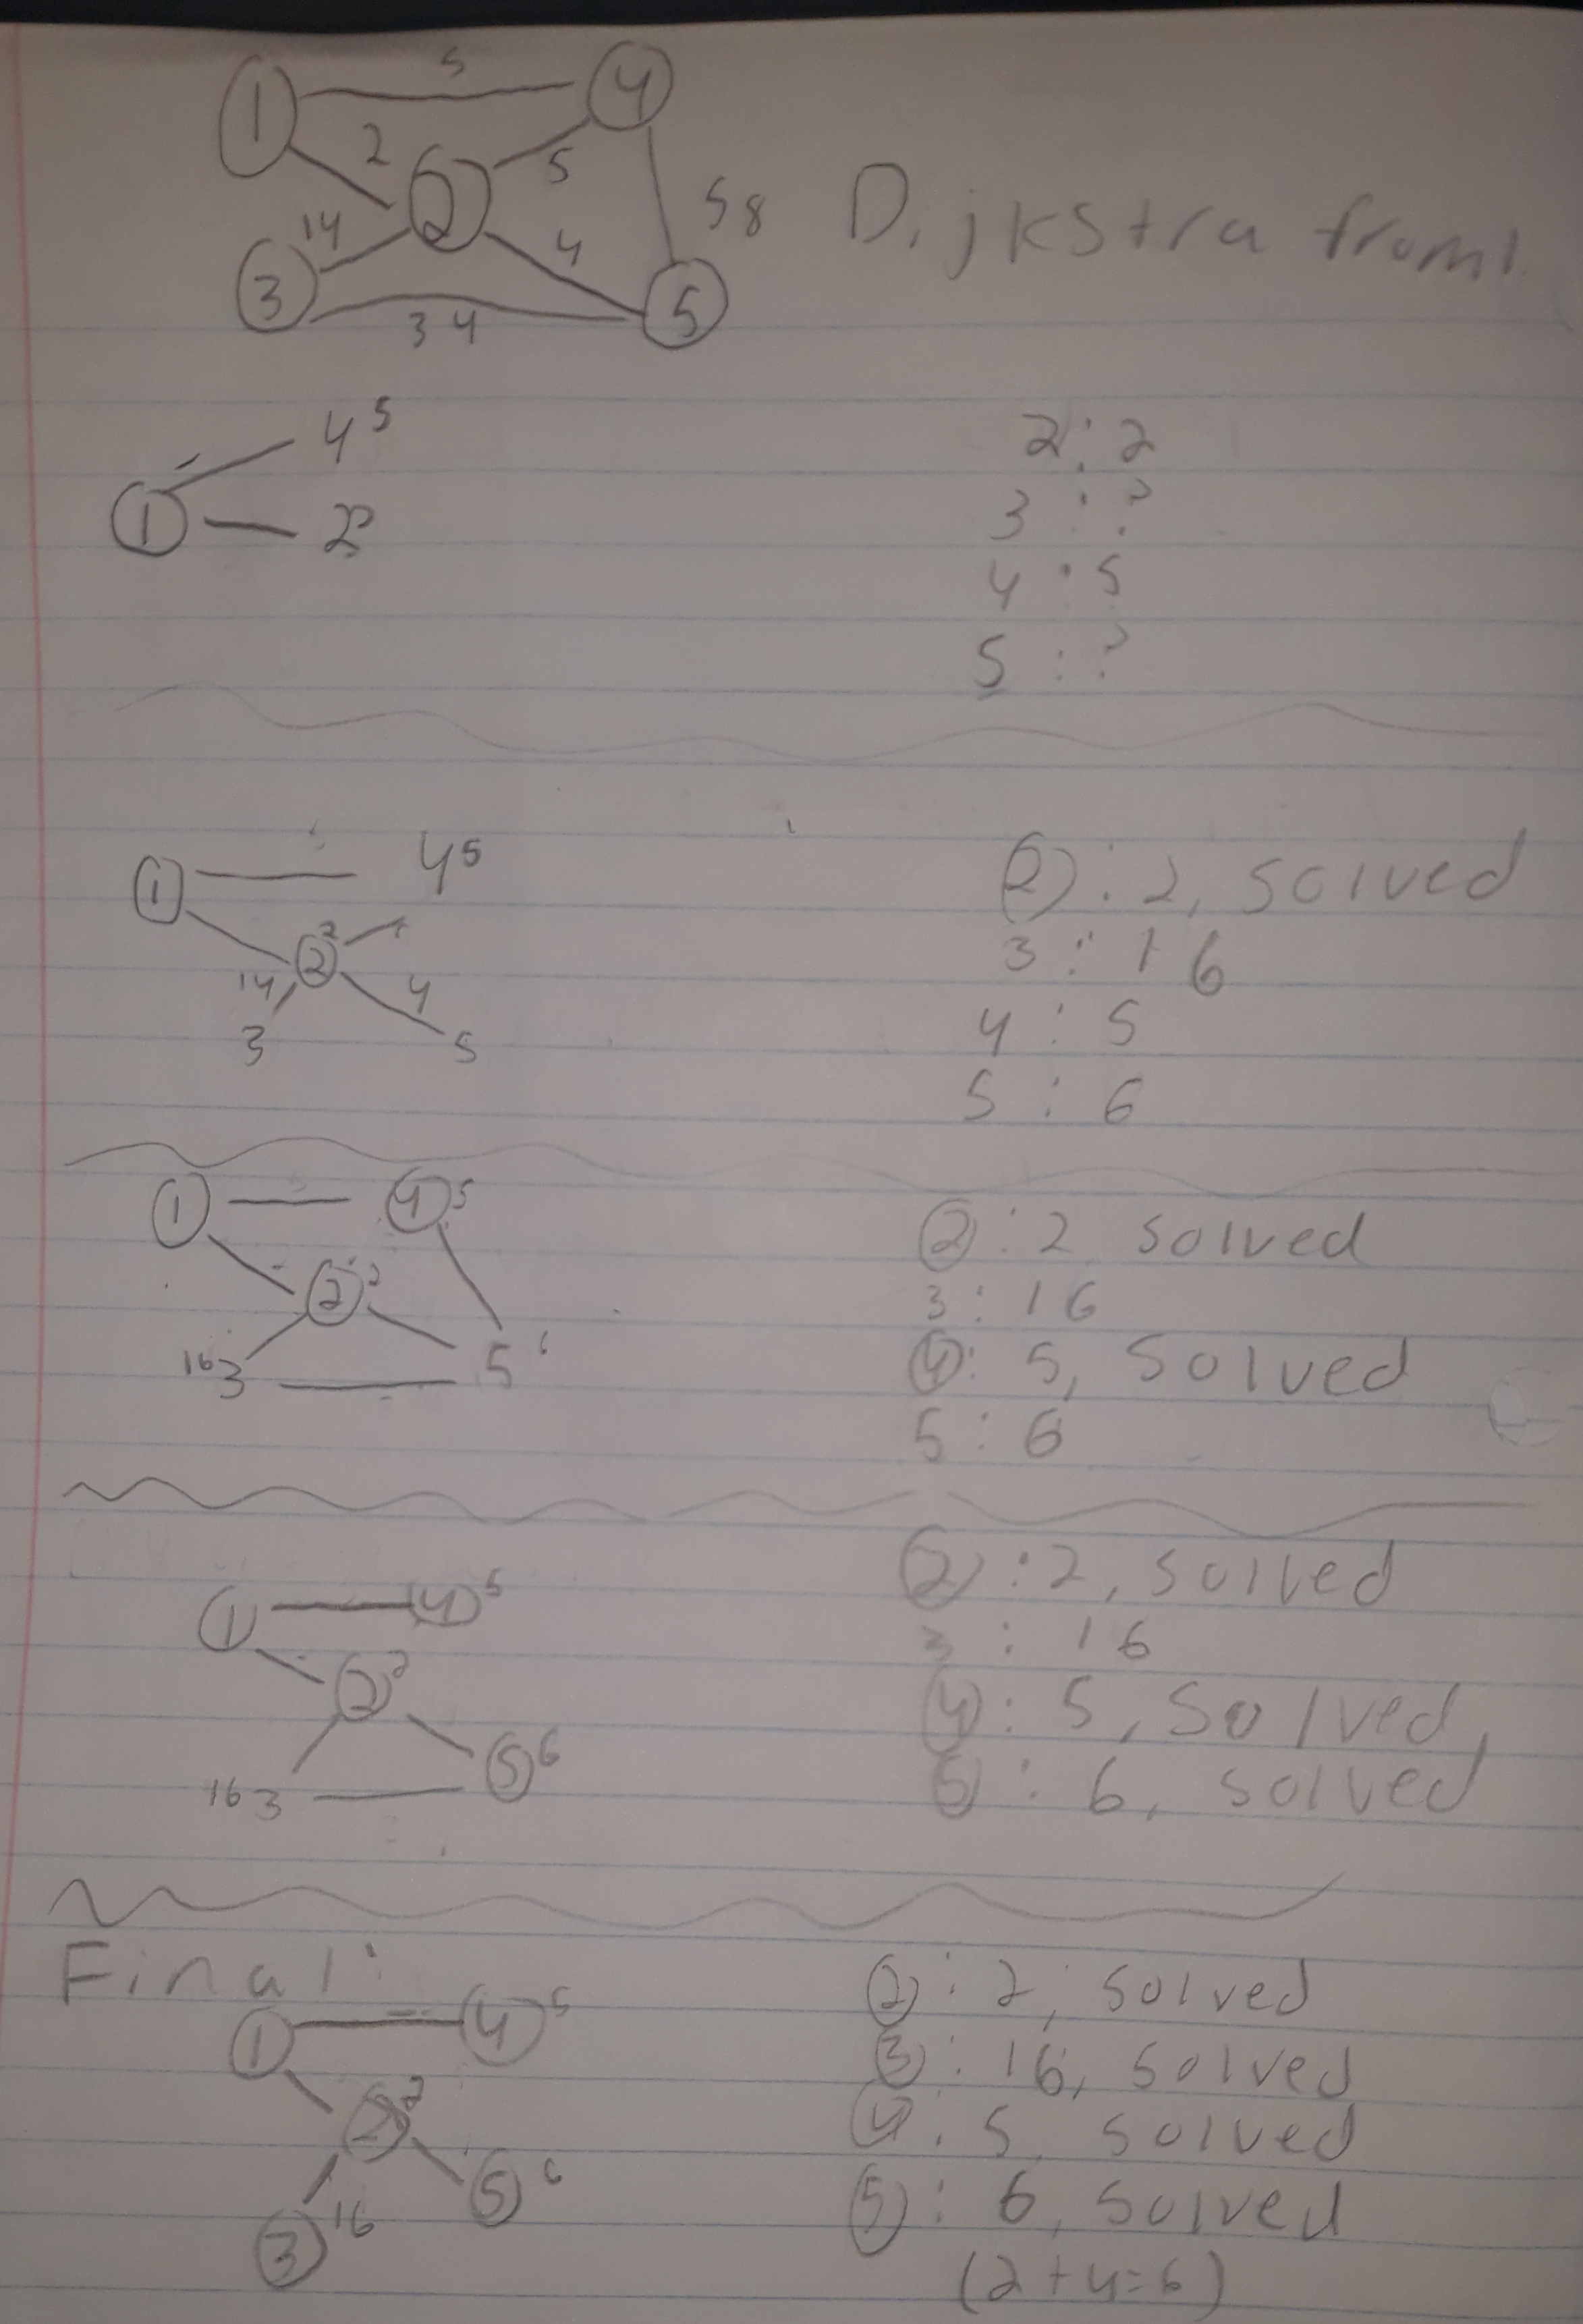
\includegraphics[width=\textwidth, height=7.5in]{Dijkstra2}$ 
\end{solution}
\pagebreak


\item (2 pts) Run Kruskal's algorithm on this graph to obtain a minimum spanning tree.
\begin{solution}
$\newline$$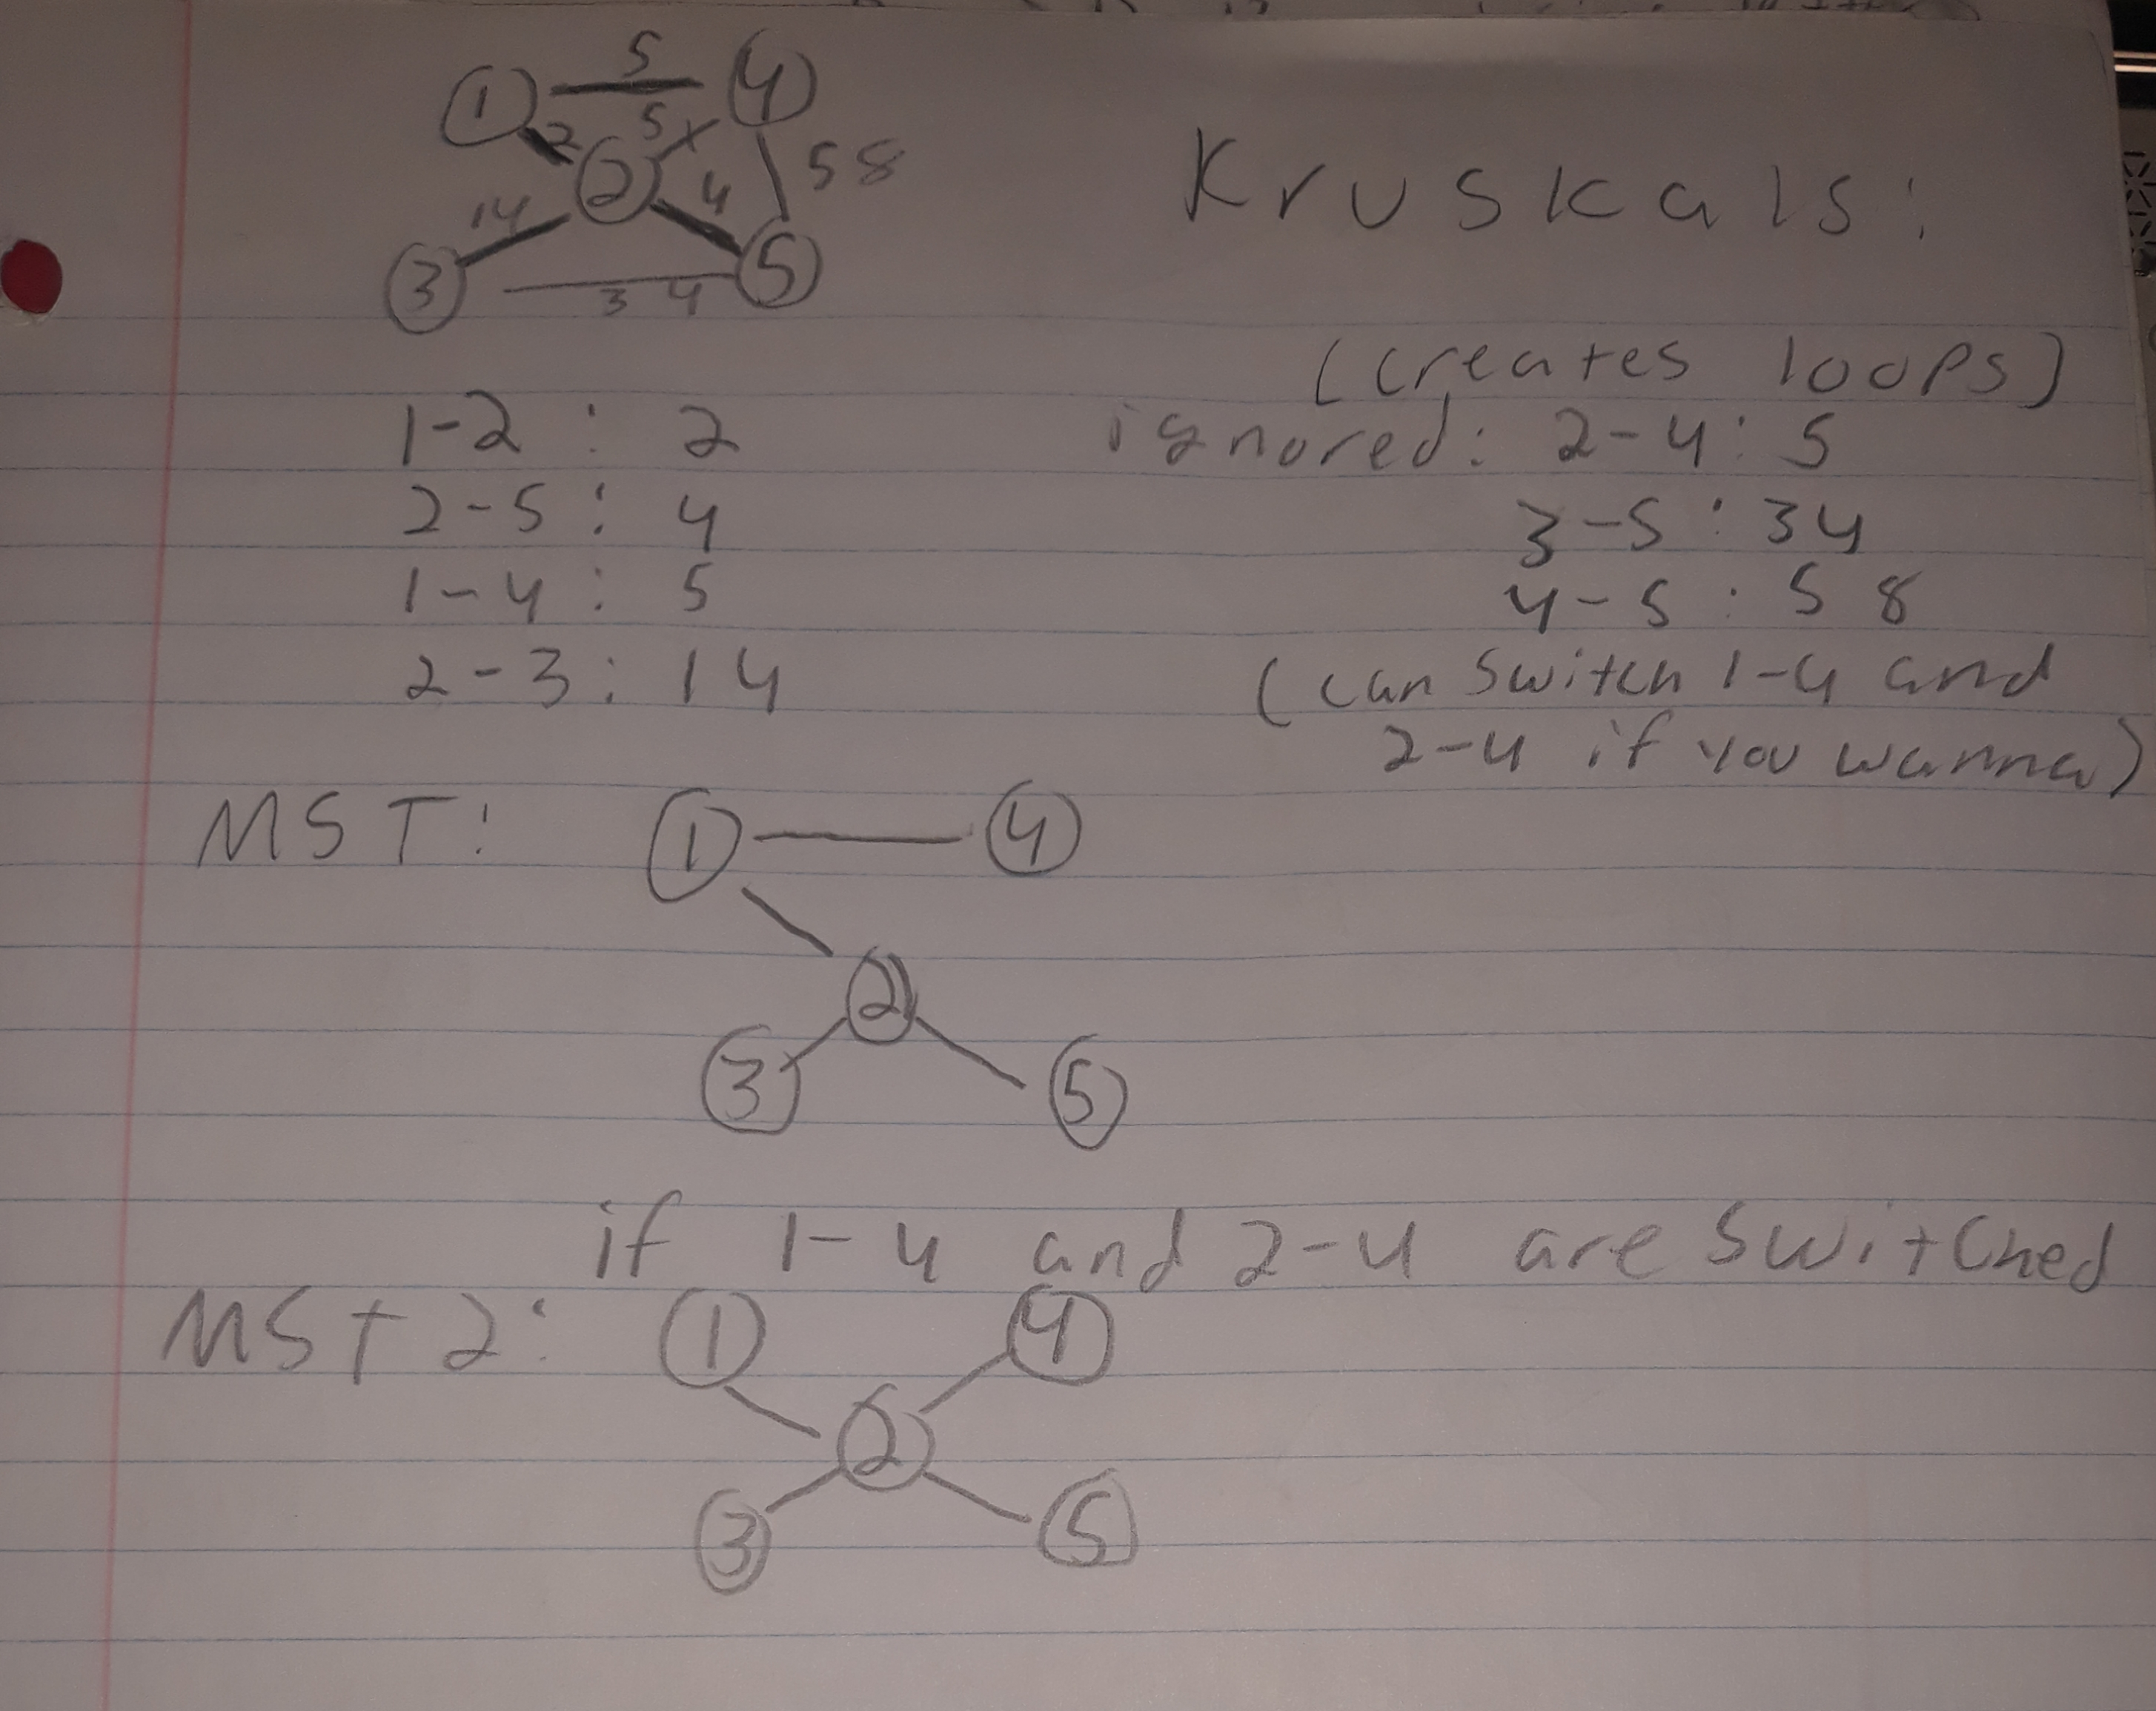
\includegraphics[width=\textwidth]{Krust}$ 
\end{solution}


\item (1 pts) Is the tree of shortest paths produced by Dijkstra's algorithm a minimum spanning tree? Justify your answer.
\begin{solution}
$\newline$ The shortest path Dijkstra did produce a minimum spanning tree. Not only does it look exactly like the first Krustal tree, but it also takes the shortest edge lengths to create the shortest paths, which algorithms actively look for to make an MST.
\end{solution}
 $\pagebreak$

\item (2 pts) Find two vertices $u$ and $v$, where the $u-v$ path in the Kruskal tree is not a shortest $u-v$ path.
\begin{solution}
$\newline$ Using the Kruskals MST2 above, the 1-4 path is not the shortest path. This specific MST uses the 2-4 path instead of the 1-4 path to get to 4, which means this minimum spanning tree makes 1-2 a necessity and automatically adds 2 to the path, making the path 7 instead of 5.
\end{solution}

\end{enumerate}

\pagebreak
\item (1 pt) Provide a brief description of what the \textit{find(v)} and \textit{union(A,B)} features of the union-find algorithm produce. 
\begin{solution}
$\newline \textit{find(v)}$: This looks at the specific vertex to find the leader of the connected component, telling which component the vertex is a part of. $\newline  \textit{union(A,B)}$: This connects two components to make a bigger connected component.
\end{solution}

\item (3 pts) Identify three edges in the following graph $G$ that won't be included in any MST of $G$. Provide a 3-4 sentence explanation of your answer.  
\begin{figure}[h!]
\begin{center}
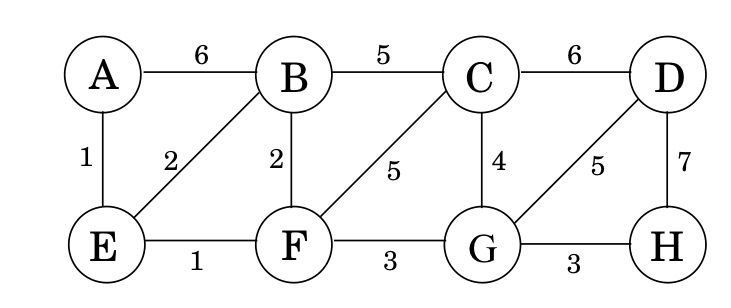
\includegraphics[scale=0.3]{mst_graph_q2.jpg} 
\end{center}
\end{figure}
\begin{solution}
$\newline$ The edges DH, CD, and AB will never be used in a minimum spanning tree. First off, compared to the values around them (especially AB), these values hold the highest weights. In addition, in looking at the MST's created with this in previous homeworks, we can get a minimum limiting edge of 5 from side GD, which is the best path to D compared to the two other ones that enter into D (being the DH and CD we are looking at now). Since all three of these are greater than the limiting edge of 5, and all MSTs are MLTs, these values cannot be in a minimum spanning tree.
\end{solution}


\end{enumerate}

\end{document}
